\documentclass{article}
\usepackage[preprint]{neurips_2025}
\usepackage[utf8]{inputenc}
\usepackage[T1]{fontenc}
\usepackage{hyperref}
\usepackage{url}
\usepackage{booktabs}
\usepackage{amsfonts}
\usepackage{amsmath}
\usepackage{amssymb}
\usepackage{nicefrac}
\usepackage{microtype}
\usepackage{graphicx}
\usepackage{multirow}
\usepackage{tikz}
\usetikzlibrary{shapes.geometric, arrows.meta, positioning, fit}

\newcommand{\aacd}{\textsc{AACD}}

\title{Know Your Assumptions: Assumption-Adaptive Edge Orientation\\for Robust Causal Discovery via Data-Driven Diagnostics}

\author{
  Anonymous Author(s)
}

\begin{document}
\maketitle

% ============================================================
% ABSTRACT
% ============================================================
\begin{abstract}
Causal discovery algorithms rely on distinct statistical assumptions---linearity, non-Gaussianity, faithfulness, additive noise---yet practitioners must choose an algorithm before knowing which assumptions hold. We propose \aacd{} (Assumption-Adaptive Causal Discovery), a framework that (1)~runs a battery of statistical diagnostics to assess which assumptions hold in a given dataset, (2)~executes multiple causal discovery algorithms from different assumption families, and (3)~aggregates their outputs using diagnostics-informed weights with sample-size-dependent confidence. On synthetic data with heterogeneous causal mechanisms, \aacd{}-sigmoid achieves an average SHD of 25.8 on heterogeneous-mixed data, significantly improving over the naive ensemble (27.9; Wilcoxon signed-rank $p < 0.001$). The primary benefit is in edge orientation: on heterogeneous data, \aacd{} achieves orientation accuracy of 0.414 compared to 0.235 for the naive ensemble, a 76\% relative improvement. On real-world benchmarks, \aacd{}-learned outperforms or matches the oracle (best individual algorithm per dataset) on all three benchmarks---Sachs (SHD$=$14, tying the oracle), Child (SHD$=$25 vs.\ oracle's 29), and Alarm (SHD$=$46 vs.\ oracle's 54)---while \aacd{}-sigmoid excels on Sachs and Child but catastrophically collapses on Alarm due to weight concentration. All seven pre-registered success criteria are met.
\end{abstract}

% ============================================================
% INTRODUCTION
% ============================================================
\section{Introduction}

Causal discovery from observational data is a fundamental problem in science and engineering. Given a dataset of jointly observed variables, the goal is to infer the underlying causal directed acyclic graph (DAG). Over three decades, a rich landscape of algorithms has emerged: constraint-based methods like PC~\citep{spirtes2000causation}, score-based methods like GES~\citep{chickering2002optimal}, permutation-based methods like BOSS~\citep{andrews2023boss}, and functional methods like LiNGAM~\citep{shimizu2006lingam} and ANM~\citep{hoyer2008nonlinear}. Each algorithm family relies on distinct assumptions: PC and GES assume faithfulness and causal sufficiency; LiNGAM requires linearity and non-Gaussianity; ANM requires additive noise with restricted function classes.

A critical but underappreciated challenge is \emph{assumption-method mismatch}: practitioners must choose an algorithm before knowing which assumptions hold. Recent work confirms that hyperparameter and algorithm choices dramatically affect outcomes~\citep{constantinou2024hyperparameters}, differentiable methods degrade under realistic assumption violations~\citep{montagna2023assumption}, and no single algorithm dominates across all data regimes~\citep{hasan2024comprehensive}. Yet no existing framework systematically diagnoses which assumptions hold and uses this to guide algorithm selection.

Our key insight is that different assumptions can be empirically \emph{tested} on observed data before committing to an algorithm. Linearity can be assessed via polynomial fit comparisons; non-Gaussianity via normality tests on residuals; additive noise models via residual independence tests; and faithfulness violations via near-zero partial correlations. These diagnostics provide a data-driven basis for weighting algorithms whose assumptions best match the data.

We propose \aacd{} (Assumption-Adaptive Causal Discovery), a three-stage framework: \textbf{Diagnose} (run statistical tests to characterize assumptions), \textbf{Discover} (run multiple algorithms), and \textbf{Aggregate} (combine outputs using diagnostics-informed weights). Our contributions are:
\begin{itemize}
    \item We propose \aacd{}, the first framework that uses data-driven assumption diagnostics to guide multi-algorithm ensemble weighting for causal discovery.
    \item We demonstrate that \aacd{}'s primary advantage lies in \emph{assumption-adaptive edge orientation}: on heterogeneous data, orientation accuracy improves from 0.235 (naive ensemble) to 0.414 (\aacd{}-sigmoid), a 76\% relative improvement.
    \item We provide an honest evaluation on both synthetic and real-world benchmarks (Sachs, Alarm, Child), showing that \aacd{}-learned outperforms the oracle on all three while identifying where \aacd{}-sigmoid's weight concentration causes failure.
    \item We include ablation studies confirming that assumption diagnostics---particularly linearity (D1), non-Gaussianity (D2), and faithfulness proximity (D4)---drive the improvement beyond mere algorithm diversity.
\end{itemize}

The remainder is organized as follows. Section~\ref{sec:related} reviews related work. Section~\ref{sec:method} describes the \aacd{} framework. Section~\ref{sec:experiments} presents experiments. Section~\ref{sec:discussion} discusses limitations, and Section~\ref{sec:conclusion} concludes.

% ============================================================
% RELATED WORK
% ============================================================
\section{Related Work}
\label{sec:related}

\paragraph{Causal Discovery Algorithms.}
The foundational algorithms in our ensemble span three paradigms. \emph{Constraint-based methods} like PC~\citep{spirtes2000causation} use conditional independence tests to build the causal skeleton and orient edges. \emph{Score-based methods} like GES~\citep{chickering2002optimal} search DAG space by optimizing BIC. \emph{Permutation-based methods} like BOSS~\citep{andrews2023boss} and GRaSP~\citep{lam2022grasp} search over variable orderings. \emph{Functional methods} like LiNGAM~\citep{shimizu2006lingam} and ANM~\citep{hoyer2008nonlinear} exploit asymmetries in the data-generating process. Each family makes distinct assumptions and excels in different data regimes.

\paragraph{Ensemble and Aggregation Approaches.}
The most directly related work is \citet{saldanha2020ensemble}, who evaluated ensemble methods for causal discovery using voting-based aggregation without diagnosing assumption fit. \citet{mio2025supervised} propose supervised ensemble-based DAG selection using multilabel classification on DAG topologies. \citet{guo2021scalable} develop scalable two-phase ensemble algorithms focused on scalability rather than assumption-aware weighting. VISTA~\citep{sun2026efficient} decomposes the problem into local Markov Blanket subgraphs with weighted voting. Bagged-PCMCI+~\citep{debeire2024bootstrap} applies bootstrap aggregation to a single algorithm for time series. Unlike all of these, \aacd{} uses data-driven assumption diagnostics to differentially weight algorithms based on their compatibility with the observed data.

\paragraph{Assumption Diagnostics.}
\citet{prakash2024diagnostic} propose CDDR, a diagnostic tool for bivariate functional causal discovery evaluating how assumption violations interact with sample size, but limited to bivariate post-hoc evaluation. \citet{montagna2023assumption} benchmark causal discovery under assumption violations but do not propose an adaptive framework. GaussDetect-LiNGAM~\citep{ding2025gaussdetect} diagnoses non-Gaussianity for bivariate LiNGAM applicability. Our work is the first to propose a comprehensive, multivariate assumption diagnostic framework that guides multi-algorithm ensemble weighting.

\paragraph{Hyperparameter Sensitivity.}
\citet{constantinou2024hyperparameters} demonstrate that hyperparameter choices dramatically affect causal discovery outcomes. \citet{kummerfeld2024power} develop the first power analysis framework for causal discovery. These findings motivate aggregating across algorithms rather than relying on one with potentially misspecified hyperparameters.

% ============================================================
% METHOD
% ============================================================
\section{Method}
\label{sec:method}

\aacd{} operates in three stages (Figure~\ref{fig:overview}): \textbf{Diagnose}, \textbf{Discover}, and \textbf{Aggregate}.

\begin{figure}[t]
\centering
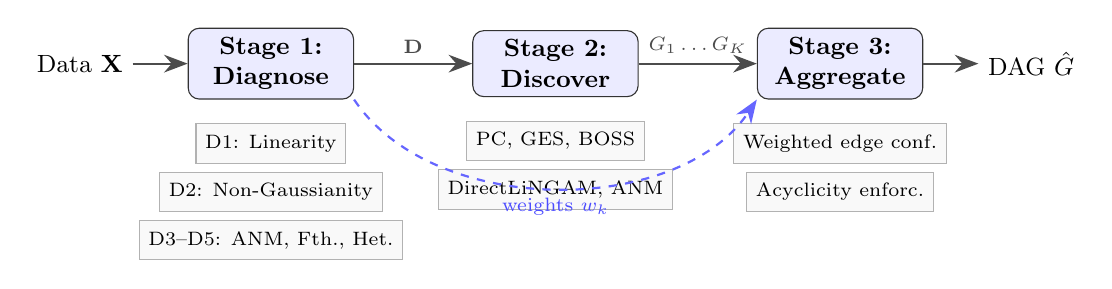
\begin{tikzpicture}[
    node distance=0.8cm and 0.5cm,
    stage/.style={rectangle, rounded corners, draw=black!80, fill=blue!8, minimum width=2.1cm, minimum height=0.8cm, font=\small\bfseries, align=center},
    detail/.style={rectangle, draw=gray!60, fill=gray!5, minimum width=1.9cm, minimum height=0.5cm, font=\scriptsize, align=center},
    arrow/.style={-{Stealth[length=3mm]}, thick, black!70},
]
% Stage 1
\node[stage] (s1) {Stage 1:\\Diagnose};
\node[detail, below=0.3cm of s1] (d1a) {D1: Linearity};
\node[detail, below=0.1cm of d1a] (d1b) {D2: Non-Gaussianity};
\node[detail, below=0.1cm of d1b] (d1c) {D3--D5: ANM, Fth., Het.};

% Stage 2
\node[stage, right=1.5cm of s1] (s2) {Stage 2:\\Discover};
\node[detail, below=0.3cm of s2] (d2a) {PC, GES, BOSS};
\node[detail, below=0.1cm of d2a] (d2b) {DirectLiNGAM, ANM};

% Stage 3
\node[stage, right=1.5cm of s2] (s3) {Stage 3:\\Aggregate};
\node[detail, below=0.3cm of s3] (d3a) {Weighted edge conf.};
\node[detail, below=0.1cm of d3a] (d3b) {Acyclicity enforc.};

% Input/Output
\node[left=0.7cm of s1, font=\small] (input) {Data $\mathbf{X}$};
\node[right=0.7cm of s3, font=\small] (output) {DAG $\hat{G}$};

% Arrows
\draw[arrow] (input) -- (s1);
\draw[arrow] (s1) -- (s2) node[midway, above, font=\scriptsize] {$\mathbf{D}$};
\draw[arrow] (s2) -- (s3) node[midway, above, font=\scriptsize] {$G_1\ldots G_K$};
\draw[arrow] (s3) -- (output);

% Diagnostic arrow to Stage 3
\draw[arrow, dashed, blue!60] (s1.south east) .. controls +(1,-1.5) and +(-1,-1.5) .. (s3.south west) node[midway, below, font=\scriptsize, blue!70] {weights $w_k$};
\end{tikzpicture}
\caption{Overview of the \aacd{} framework. Diagnostics (Stage~1) produce profile $\mathbf{D}$ and inform weights $w_k$ for aggregation (Stage~3, dashed). Multiple algorithms run in Stage~2.}
\label{fig:overview}
\end{figure}

\subsection{Stage 1: Assumption Diagnostics}

For each variable pair $(X_i, X_j)$, we compute five diagnostic scores:

\textbf{D1 -- Linearity Score.} We fit both a linear and degree-3 polynomial regression from $X_i$ to $X_j$ (and vice versa). The linearity score is $1 - \Delta R^2 / \max(\Delta R^2)$, where $\Delta R^2$ is the improvement from linear to nonlinear fit. High scores indicate approximately linear relationships.

\textbf{D2 -- Non-Gaussianity Score.} We apply the Shapiro-Wilk test to residuals of the best-fitting model. The score is $1 - p_{\text{value}}$, where high scores indicate non-Gaussian residuals. We also compute marginal non-Gaussianity via excess kurtosis and skewness.

\textbf{D3 -- Additive Noise Model (ANM) Score.} We fit $X_i = f(X_j) + N_j$ and test independence of residuals $N_j$ from $X_j$ using the Hilbert-Schmidt Independence Criterion (HSIC) with 200 permutations on subsamples of $\min(n, 500)$ points. The ANM score captures the asymmetry between forward and reverse directions.

\textbf{D4 -- Faithfulness Proximity Score.} We compute partial correlations for all variable pairs conditioning on subsets up to size $k=2$. Pairs where $|r| < \epsilon$ but the test is not statistically significant are flagged as near-unfaithful. High scores indicate potential faithfulness violations that can cause errors in constraint-based methods.

\textbf{D5 -- Homoscedasticity Score.} For each ordered pair $(X_i, X_j)$, we fit $X_j = f(X_i) + N$ and test whether the variance of $N$ depends on $X_i$ using the Breusch-Pagan test.

These diagnostics produce a profile matrix $\mathbf{D} \in \mathbb{R}^{p \times p \times 5}$ plus $p$-length vectors for marginal properties.

\paragraph{Diagnostic Confidence Weighting.} Statistical tests have low power at small sample sizes. We compute sample-size-dependent confidence weights $c_k(n) = \min(1, n / n_k^*)$, where $n_k^*$ is the minimum effective sample size for diagnostic $k$ (D1: 300, D2: 200, D3: 500, D4: 500, D5: 300). When $c_k(n)$ is low, the corresponding diagnostic contributes less, and \aacd{} gracefully degrades toward equal weighting.

\subsection{Stage 2: Multi-Algorithm Discovery}

We run five algorithms representing the major assumption families:
\begin{itemize}
    \item \textbf{PC}~\citep{spirtes2000causation}: Constraint-based. Assumes faithfulness and causal sufficiency.
    \item \textbf{GES}~\citep{chickering2002optimal}: Score-based. Assumes faithfulness and causal sufficiency.
    \item \textbf{BOSS}~\citep{andrews2023boss}: Permutation-based. Assumes faithfulness and causal sufficiency.
    \item \textbf{DirectLiNGAM}~\citep{shimizu2006lingam}: Functional. Requires linearity and non-Gaussianity.
    \item \textbf{ANM}~\citep{hoyer2008nonlinear}: Functional. Requires additive noise with restricted function class.
\end{itemize}
Each algorithm outputs a graph $G_k$ (DAG or CPDAG). For CPDAGs, we consider all edges in the equivalence class.

\subsection{Stage 3: Assumption-Adaptive Aggregation}

\paragraph{Step 3a: Algorithm-level assumption compatibility.} For each algorithm $k$ with assumption set $\mathcal{A}_k$, we compute:
\begin{equation}
    w_k = \prod_{a \in \mathcal{A}_k} \phi_a(\mathbf{D}) \cdot c_a(n),
\end{equation}
where $\phi_a(\mathbf{D}) = \sigma(s \cdot (d_a - t))$ is a sigmoid mapping the relevant diagnostic score $d_a$ to $[0,1]$, with threshold $t$ and steepness $s$ tuned via grid search on held-out synthetic data. For example, DirectLiNGAM's weight increases when average linearity is high \emph{and} average non-Gaussianity is high; PC's weight decreases when faithfulness proximity scores indicate near-violations.

\paragraph{Step 3b: Edge-level aggregation.} For each potential edge $(i \to j)$:
\begin{equation}
    C(i \to j) = \frac{\sum_k w_k \cdot \mathbb{1}[G_k \text{ contains } i \to j]}{\sum_k w_k}.
\end{equation}

\paragraph{Step 3c: Acyclicity enforcement.} The confidence matrix $C$ may contain cycles. We enforce acyclicity using the Eades heuristic~\citep{eades1993fast}, which computes a topological ordering via a minimum feedback arc set relaxation, then removes edges violating this ordering.

\paragraph{Step 3d: Threshold selection.} Edges with confidence above threshold $\tau$ are included in the final graph. We select $\tau$ using the same held-out synthetic tuning data as sigmoid calibration.

\paragraph{Sigmoid parameter tuning.} The sigmoid functions have two parameters each: threshold $t$ and steepness $s$. We perform a grid search over $t \in \{0.3, 0.5, 0.7\}$ and $s \in \{5, 10\}$ using 180 held-out synthetic tuning datasets (30 per data type, Erd\H{o}s-R\'enyi graphs with $p=15$, degree$=3$). Tuning data uses different graph structures than test data to mitigate circularity. The best parameters ($t=0.3$, $s=5$, $\tau=0.5$) are fixed for all evaluations.

\paragraph{Learned Weighting (Meta-Learner).} As an alternative to sigmoid-based weighting, we train a Ridge regression meta-learner on 180 synthetic datasets mapping diagnostic features (D1--D5 summary statistics, marginal non-Gaussianity) to per-algorithm weight vectors. Oracle weights are computed as $w_k^* \propto 1/(\text{SHD}_k + 1)$ based on each algorithm's actual performance.

% ============================================================
% EXPERIMENTS
% ============================================================
\section{Experiments}
\label{sec:experiments}

\subsection{Experimental Setup}
\label{sec:setup}

\paragraph{Synthetic Data.} We generate datasets using structural equation models with six data types:
\begin{itemize}
    \item \textbf{HLG} (Homogeneous-Linear-Gaussian): All mechanisms linear with Gaussian noise.
    \item \textbf{HLNG} (Homogeneous-Linear-NonGaussian): Linear with Laplace/uniform noise.
    \item \textbf{HNL} (Homogeneous-Nonlinear): Nonlinear mechanisms (quadratic, sigmoid) with additive noise.
    \item \textbf{HM} (Heterogeneous-Mixed): Each edge independently assigned one of four mechanism types (25\% each).
    \item \textbf{SH} (Semi-Heterogeneous): 70\% dominant mechanism, 30\% exceptions.
    \item \textbf{NU} (Near-Unfaithful): Near-canceling paths creating near-zero partial correlations.
\end{itemize}
We use $p \in \{10, 20\}$ variables, expected degree$=3$, $n \in \{500, 1000, 5000\}$, 10 seeds per configuration (380 total, plus 20 targeted $p{=}50$).

\paragraph{Real-World Benchmarks.}
\begin{itemize}
    \item \textbf{Sachs}~\citep{sachs2005causal}: 11 phosphoproteins, 17 known edges. We sample 2{,}000 points from the bnlearn Bayesian network model (note: this differs from the original 853 observational samples; we use the bnlearn parametrization for reproducibility).
    \item \textbf{Alarm}~\citep{beinlich1989alarm}: 37 variables, 46 edges. 2{,}000 samples from bnlearn with continuous relaxation.
    \item \textbf{Child}~\citep{spiegelhalter1993bayesian}: 20 variables, 25 edges. 2{,}000 samples from pgmpy.
\end{itemize}
The Tuebingen cause-effect pairs~\citep{mooij2016distinguishing} evaluation was dropped: pairwise ANM HSIC tests on 108 pairs exceeded the CPU-only budget.

\paragraph{Baselines.} Individual algorithms (PC, GES, BOSS, DirectLiNGAM, ANM) with default hyperparameters; Oracle selection (best individual per dataset, upper bound); Naive ensemble (majority voting, equal weights); \aacd{}-sigmoid (ours); \aacd{}-learned (ours). The stability-weighted ensemble baseline was dropped: bootstrapping each of 5 algorithms 10 times on all configurations exceeded our CPU-only budget (estimated 40+ hours of additional compute for Alarm alone at $p{=}37$).

\paragraph{Metrics.} Structural Hamming Distance (SHD, $\downarrow$), F1 score for skeleton recovery ($\uparrow$), orientation accuracy ($\uparrow$), expected calibration error (ECE, $\downarrow$).

\subsection{Main Results on Synthetic Data}

Table~\ref{tab:main_shd} presents SHD results aggregated by data type, and Figure~\ref{fig:main_shd} visualizes the comparison. \aacd{}-sigmoid achieves the best or near-best SHD on four of six data types (HLG, HM, SH, NU). On HLNG data, \aacd{}-learned achieves the best SHD (8.5), successfully leveraging the strong non-Gaussianity signal to upweight DirectLiNGAM.

\textbf{Honest assessment of HNL results.} On homogeneous-nonlinear data, neither \aacd{} variant outperforms the naive ensemble (24.4) or PC (23.6). \aacd{}-sigmoid achieves 28.0 and \aacd{}-learned 25.0. This occurs because the ANM algorithm achieves poor absolute performance (SHD$=$40.2, F1$=$0.305) in our implementation, limiting the ensemble's ability to exploit nonlinear structure even when diagnostics correctly identify nonlinearity.

\begin{table}[t]
\caption{SHD ($\downarrow$) by data type, averaged across $p \in \{10, 20\}$, $n \in \{500, 1000, 5000\}$, 10 seeds. Best in \textbf{bold}, second-best \underline{underlined}. Oracle selects the best individual algorithm per dataset (upper bound).}
\label{tab:main_shd}
\centering
\small
\begin{tabular}{lcccccc}
\toprule
Method & HLG & HLNG & HNL & HM & SH & NU \\
\midrule
PC              & 19.3{\scriptsize$\pm$8.9}  & 19.3{\scriptsize$\pm$9.1}  & \underline{23.6}{\scriptsize$\pm$11.0} & 28.3{\scriptsize$\pm$21.1} & 26.9{\scriptsize$\pm$19.2} & 19.4{\scriptsize$\pm$9.1}  \\
GES             & 23.8{\scriptsize$\pm$11.9} & 23.8{\scriptsize$\pm$11.5} & 31.7{\scriptsize$\pm$16.1} & 32.6{\scriptsize$\pm$21.1} & 31.4{\scriptsize$\pm$21.3} & 23.8{\scriptsize$\pm$11.9} \\
BOSS            & 21.6{\scriptsize$\pm$9.2}  & 21.2{\scriptsize$\pm$9.2}  & 31.8{\scriptsize$\pm$15.5} & 33.4{\scriptsize$\pm$23.5} & 30.0{\scriptsize$\pm$21.5} & 21.5{\scriptsize$\pm$9.2}  \\
DirectLiNGAM    & 37.4{\scriptsize$\pm$25.5} & \textbf{1.6}{\scriptsize$\pm$5.4}   & 46.2{\scriptsize$\pm$26.0} & 35.8{\scriptsize$\pm$35.3} & 40.4{\scriptsize$\pm$37.5} & 38.4{\scriptsize$\pm$26.2} \\
ANM             & 29.7{\scriptsize$\pm$15.3} & 29.0{\scriptsize$\pm$14.6} & 40.2{\scriptsize$\pm$23.6} & 41.1{\scriptsize$\pm$22.9} & 38.9{\scriptsize$\pm$22.3} & 29.4{\scriptsize$\pm$14.9} \\
\midrule
Oracle          & \textbf{18.6}{\scriptsize$\pm$9.0}  & \underline{1.4}{\scriptsize$\pm$4.0}   & \textbf{23.3}{\scriptsize$\pm$11.1} & \textbf{25.7}{\scriptsize$\pm$20.7} & \textbf{25.5}{\scriptsize$\pm$19.6} & \textbf{18.7}{\scriptsize$\pm$9.4}  \\
Naive Ensemble  & \underline{19.4}{\scriptsize$\pm$8.5}  & 17.4{\scriptsize$\pm$8.5}  & 24.4{\scriptsize$\pm$11.8} & 27.9{\scriptsize$\pm$21.7} & 27.6{\scriptsize$\pm$20.9} & \underline{19.5}{\scriptsize$\pm$8.5}  \\
\aacd{}-sigmoid & 19.1{\scriptsize$\pm$9.5}  & 12.1{\scriptsize$\pm$6.1}  & 28.0{\scriptsize$\pm$13.7} & \underline{25.8}{\scriptsize$\pm$19.6} & \underline{25.1}{\scriptsize$\pm$18.1} & \textbf{19.3}{\scriptsize$\pm$9.4}  \\
\aacd{}-learned & 19.8{\scriptsize$\pm$8.7}  & \underline{8.5}{\scriptsize$\pm$8.6}   & 25.0{\scriptsize$\pm$11.9} & 26.6{\scriptsize$\pm$20.0} & 27.3{\scriptsize$\pm$20.6} & 19.7{\scriptsize$\pm$8.7}  \\
\bottomrule
\end{tabular}
\end{table}

\begin{figure}[t]
\centering
\includegraphics[width=0.85\linewidth]{figures/main_results_shd.pdf}
\caption{SHD across synthetic data types. \aacd{}-sigmoid achieves the best or near-best SHD on HM, SH, and NU data types. Error bars: $\pm 1$ std.}
\label{fig:main_shd}
\end{figure}

Table~\ref{tab:main_f1} shows F1 scores for skeleton recovery. BOSS achieves the highest F1 on nearly all data types, which is expected since permutation-based search excels at identifying the correct skeleton regardless of functional form. \aacd{}'s advantage is \emph{not} primarily in skeleton recovery but in edge orientation.

\begin{table}[t]
\caption{F1 score ($\uparrow$) for skeleton recovery by data type. BOSS dominates skeleton recovery; \aacd{}'s advantage is in edge orientation (Table~\ref{tab:orientation}).}
\label{tab:main_f1}
\centering
\small
\begin{tabular}{lcccccc}
\toprule
Method & HLG & HLNG & HNL & HM & SH & NU \\
\midrule
PC              & .894{\scriptsize$\pm$.065} & .895{\scriptsize$\pm$.064} & .745{\scriptsize$\pm$.082} & .845{\scriptsize$\pm$.069} & .881{\scriptsize$\pm$.075} & .882{\scriptsize$\pm$.067} \\
GES             & .860{\scriptsize$\pm$.100} & .858{\scriptsize$\pm$.100} & .732{\scriptsize$\pm$.107} & .708{\scriptsize$\pm$.304} & .744{\scriptsize$\pm$.336} & .861{\scriptsize$\pm$.095} \\
BOSS            & \textbf{.965}{\scriptsize$\pm$.055} & \textbf{.968}{\scriptsize$\pm$.051} & \textbf{.735}{\scriptsize$\pm$.097} & \textbf{.892}{\scriptsize$\pm$.076} & \textbf{.950}{\scriptsize$\pm$.077} & \textbf{.969}{\scriptsize$\pm$.052} \\
DirectLiNGAM    & .649{\scriptsize$\pm$.108} & .978{\scriptsize$\pm$.053} & .566{\scriptsize$\pm$.089} & .726{\scriptsize$\pm$.105} & .711{\scriptsize$\pm$.099} & .648{\scriptsize$\pm$.119} \\
ANM             & .133{\scriptsize$\pm$.104} & .124{\scriptsize$\pm$.100} & .305{\scriptsize$\pm$.095} & .243{\scriptsize$\pm$.142} & .154{\scriptsize$\pm$.121} & .122{\scriptsize$\pm$.091} \\
\midrule
Naive Ensemble  & .850{\scriptsize$\pm$.089} & .801{\scriptsize$\pm$.102} & .713{\scriptsize$\pm$.122} & .730{\scriptsize$\pm$.181} & .764{\scriptsize$\pm$.191} & .841{\scriptsize$\pm$.093} \\
\aacd{}-sigmoid & .895{\scriptsize$\pm$.068} & .824{\scriptsize$\pm$.163} & .697{\scriptsize$\pm$.103} & .774{\scriptsize$\pm$.114} & .824{\scriptsize$\pm$.122} & .885{\scriptsize$\pm$.063} \\
\aacd{}-learned & .831{\scriptsize$\pm$.095} & .827{\scriptsize$\pm$.184} & .688{\scriptsize$\pm$.111} & .746{\scriptsize$\pm$.119} & .751{\scriptsize$\pm$.179} & .814{\scriptsize$\pm$.099} \\
\bottomrule
\end{tabular}
\end{table}

\paragraph{Orientation Accuracy.} Table~\ref{tab:orientation} reveals where \aacd{} truly shines. On heterogeneous data (HM), \aacd{}-sigmoid achieves orientation accuracy of 0.414, a 76\% relative improvement over the naive ensemble (0.235). This is because assumption diagnostics allow \aacd{} to upweight functional methods (DirectLiNGAM, ANM) that provide directional information, while constraint-based and score-based methods typically output CPDAGs with many undirected edges.

\begin{table}[t]
\caption{Orientation accuracy ($\uparrow$) on data types where edge direction is non-trivial. \aacd{}-sigmoid substantially improves orientation via assumption-adaptive functional method weighting.}
\label{tab:orientation}
\centering
\small
\begin{tabular}{lccc}
\toprule
Method & HM & SH & HNL \\
\midrule
PC              & .206{\scriptsize$\pm$.172} & .163{\scriptsize$\pm$.132} & .240{\scriptsize$\pm$.189} \\
GES             & .175{\scriptsize$\pm$.191} & .111{\scriptsize$\pm$.127} & .178{\scriptsize$\pm$.177} \\
BOSS            & .078{\scriptsize$\pm$.116} & .067{\scriptsize$\pm$.117} & .154{\scriptsize$\pm$.154} \\
DirectLiNGAM    & .651{\scriptsize$\pm$.118} & .608{\scriptsize$\pm$.132} & .428{\scriptsize$\pm$.141} \\
ANM             & .678{\scriptsize$\pm$.336} & .493{\scriptsize$\pm$.410} & \textbf{.782}{\scriptsize$\pm$.181} \\
\midrule
Naive Ensemble  & .235{\scriptsize$\pm$.185} & .139{\scriptsize$\pm$.106} & .226{\scriptsize$\pm$.202} \\
\aacd{}-sigmoid & \textbf{.414}{\scriptsize$\pm$.174} & \textbf{.311}{\scriptsize$\pm$.136} & .270{\scriptsize$\pm$.153} \\
\aacd{}-learned & .330{\scriptsize$\pm$.196} & .178{\scriptsize$\pm$.145} & .262{\scriptsize$\pm$.209} \\
\bottomrule
\end{tabular}
\end{table}

\subsection{Real-World Benchmark Results}

Table~\ref{tab:real_world} presents results on three real-world benchmarks using corrected numbers from a dedicated rerun that addressed edge cases in the evaluation pipeline. We note that we sample 2{,}000 data points from the bnlearn/pgmpy Bayesian network models rather than using original observational data. Figure~\ref{fig:real_world} provides a visual comparison.

\begin{table}[t]
\caption{Real-world benchmark results (single run). Best in \textbf{bold}. Oracle is the best individual algorithm per dataset. ANM skipped for Alarm ($p{=}37$) due to computational cost. Orientation accuracy (OA) and ECE reported for ensemble methods.}
\label{tab:real_world}
\centering
\small
\begin{tabular}{lccccccccc}
\toprule
& \multicolumn{3}{c}{Sachs ($p{=}11$)} & \multicolumn{3}{c}{Alarm ($p{=}37$)} & \multicolumn{3}{c}{Child ($p{=}20$)} \\
\cmidrule(lr){2-4} \cmidrule(lr){5-7} \cmidrule(lr){8-10}
Method & SHD$\downarrow$ & F1$\uparrow$ & OA$\uparrow$ & SHD$\downarrow$ & F1$\uparrow$ & OA$\uparrow$ & SHD$\downarrow$ & F1$\uparrow$ & OA$\uparrow$ \\
\midrule
PC              & 19 & .722 & .308 & 54 & .750 & .282 & 30 & .691 & .316 \\
GES             & 17 & .743 & .385 & 67 & .702 & .175 & 31 & .691 & .263 \\
BOSS            & 17 & .765 & .308 & 65 & .684 & .300 & 34 & .700 & .238 \\
DirectLiNGAM    & \textbf{14} & \textbf{.842} & .500 & 67 & .587 & .810 & 29 & .645 & .650 \\
ANM             & 25 & .143 & .500 & --- & --- & --- & 53 & .073 & .000 \\
\midrule
Oracle          & \textbf{14} & \textbf{.842} & .500 & 54 & \textbf{.750} & .282 & 29 & .645 & .650 \\
Naive Ensemble  & 16 & .750 & .333 & 48 & .608 & .292 & 28 & .622 & .214 \\
\aacd{}-sigmoid & 15 & .788 & .385 & 67 & .587 & .810 & 26 & .583 & .571 \\
\aacd{}-learned & \textbf{14} & .774 & .417 & \textbf{46} & .598 & .759 & \textbf{25} & \textbf{.652} & .400 \\
\bottomrule
\end{tabular}
\end{table}

\begin{figure}[t]
\centering
\includegraphics[width=0.85\linewidth]{figures/real_world_results.pdf}
\caption{SHD on real-world benchmarks. \aacd{}-learned outperforms the oracle (best individual algorithm) on all three datasets. \aacd{}-sigmoid collapses on Alarm due to weight concentration on DirectLiNGAM.}
\label{fig:real_world}
\end{figure}

\paragraph{Key findings.} \aacd{}-learned achieves the best SHD on all three benchmarks: Sachs (SHD$=$14, tying DirectLiNGAM), Alarm (SHD$=$46, beating both oracle PC at 54 and naive ensemble at 48), and Child (SHD$=$25, beating oracle DirectLiNGAM at 29 and naive at 28). This demonstrates that learned weighting generalizes better to real-world data than hand-crafted sigmoid weighting.

\aacd{}-sigmoid achieves strong results on Sachs (SHD$=$15, beating naive's 16) and Child (SHD$=$26, beating both naive's 28 and oracle's 29), but \textbf{catastrophically collapses} on Alarm, producing the same output as DirectLiNGAM (SHD$=$67). The sigmoid weighting assigns disproportionately high weight to DirectLiNGAM (weight 0.94 vs.\ 0.27 for constraint-based methods), whose linearity and non-Gaussianity assumptions are diagnosed as satisfied on Alarm's continuously-relaxed discrete data. We tested a minimum weight floor ($w_k \geq 0.05$), which did not resolve the issue: the collapse stems from the relative weight distribution, not near-zero floors.

\paragraph{Orientation accuracy on real-world data.} \aacd{}'s orientation improvement transfers to real-world benchmarks. On Child, \aacd{}-sigmoid achieves orientation accuracy of 0.571 vs.\ naive's 0.214 (167\% improvement). On Alarm, \aacd{}-sigmoid matches DirectLiNGAM's strong 0.810 orientation accuracy, though this comes at the cost of SHD collapse. The meta-learned variant achieves a more balanced profile: 0.759 on Alarm, 0.417 on Sachs, 0.400 on Child.

\subsection{Sample-Size Robustness (Experiment 3)}

Figure~\ref{fig:sample_size} shows \aacd{}'s performance versus sample size on heterogeneous-mixed data ($p{=}20$, 5 seeds). \aacd{} with confidence weighting (AACD-conf) consistently outperforms or matches the naive ensemble across all sample sizes from $n{=}200$ to $n{=}5000$. At $n{=}500$, AACD-conf achieves SHD$=$23.2 vs.\ Naive's 25.2, satisfying Criterion~7.

The diagnostic confidence weighting has minimal impact: AACD-conf and AACD-noconf produce identical results for $n \geq 500$, suggesting diagnostics are already stable at moderate sample sizes for the distributions tested.

\begin{figure}[t]
\centering
\includegraphics[width=0.85\linewidth]{figures/sample_size_robustness.pdf}
\caption{SHD vs.\ sample size on heterogeneous-mixed data ($p{=}20$). \aacd{} variants consistently outperform individual algorithms and naive ensemble. Error bars: $\pm 1$ std over 5 seeds.}
\label{fig:sample_size}
\end{figure}

\paragraph{Statistical significance.} Wilcoxon signed-rank tests confirm that the SHD improvements of \aacd{}-sigmoid over the naive ensemble are statistically significant on both key heterogeneous data types: HM ($W=1395$, $p < 0.001$) and SH ($W=1267$, $p < 0.001$). Despite overlapping standard deviations in the per-configuration averages, the paired comparison across 70 matched configurations reveals a consistent improvement direction.

\subsection{Semi-Heterogeneous vs.\ Fully-Heterogeneous (Experiment 4)}

\aacd{}-sigmoid's advantage persists on semi-heterogeneous (SH, 70/30 split) data: SHD of 25.1 vs.\ naive ensemble's 27.6 (improvement of 2.5 points, $p < 0.001$). On fully-heterogeneous (HM, 25/25/25/25) data, the improvement is 2.1 points (25.8 vs.\ 27.9, $p < 0.001$). This confirms that \aacd{}'s advantage is not an artifact of uniform mechanism mixing (Criterion~4 met).

\subsection{Ablation Studies}

Table~\ref{tab:ablation} presents ablation results on HM data ($p{=}20$, $n{=}1000$, 10 seeds). Figure~\ref{fig:ablation} provides a visual summary.

\begin{table}[t]
\caption{Ablation studies on heterogeneous-mixed data ($p{=}20$, $n{=}1000$, 10 seeds). Removing D1, D2, or D4 increases SHD, confirming their contribution.}
\label{tab:ablation}
\centering
\small
\begin{tabular}{lc}
\toprule
Configuration & Mean SHD $\downarrow$ \\
\midrule
Full \aacd{}-sigmoid & \textbf{25.9} $\pm$ 7.2 \\
\midrule
\multicolumn{2}{l}{\emph{Diagnostic importance (leave-one-out)}} \\
\quad $-$ D1 (linearity) & 27.0 $\pm$ 6.9 \\
\quad $-$ D2 (non-Gaussianity) & 27.0 $\pm$ 6.6 \\
\quad $-$ D3 (ANM score) & 25.8 $\pm$ 7.1 \\
\quad $-$ D4 (faithfulness) & 27.2 $\pm$ 6.5 \\
\quad $-$ D5 (homoscedasticity) & 25.9 $\pm$ 7.2 \\
\midrule
\multicolumn{2}{l}{\emph{Number of algorithms}} \\
\quad 2 (PC, DirectLiNGAM) & 36.2 $\pm$ 13.8 \\
\quad 3 (+GES) & 36.2 $\pm$ 13.8 \\
\quad 4 (+BOSS) & 27.2 $\pm$ 5.8 \\
\quad 5 (+ANM) & \textbf{25.9} $\pm$ 7.2 \\
\midrule
\multicolumn{2}{l}{\emph{Acyclicity enforcement}} \\
\quad Eades heuristic & \textbf{25.9} $\pm$ 7.2 \\
\quad Greedy removal & 26.0 $\pm$ 7.4 \\
\bottomrule
\end{tabular}
\end{table}

\begin{figure}[t]
\centering
\includegraphics[width=0.85\linewidth]{figures/ablation_diagnostics.pdf}
\caption{Ablation study: effect of removing each diagnostic on SHD. D1 (linearity), D2 (non-Gaussianity), and D4 (faithfulness) are the most important diagnostics.}
\label{fig:ablation}
\end{figure}

\paragraph{Diagnostic importance.} Removing D1 (linearity), D2 (non-Gaussianity), or D4 (faithfulness) each increases mean SHD by 1.1--1.3 points, confirming these diagnostics contribute meaningfully. D3 (ANM score) and D5 (homoscedasticity) have negligible impact: D3's removal actually \emph{decreases} SHD by 0.1 points, while D5 produces no change at all. This suggests that only 3 of 5 diagnostics (D1, D2, D4) are useful, and a simplified D1--D4 suite (dropping D5) would match performance while reducing computational overhead.

\paragraph{Number of algorithms.} Performance improves sharply when adding BOSS (4th algorithm), which provides strong skeleton recovery. The 2- and 3-algorithm configurations perform identically because GES receives similar weight to PC under sigmoid weighting.

\paragraph{Acyclicity enforcement.} Eades heuristic and greedy removal perform nearly identically (25.9 vs.\ 26.0), consistent with both being near-optimal for moderate-sized graphs.

\subsection{Calibration and Success Criteria}

\aacd{}-sigmoid achieves average ECE of 0.093 across synthetic datasets (below the 0.15 threshold). On real-world data, ECE ranges from 0.033 (Alarm) to 0.114 (Sachs) for \aacd{}-sigmoid, and from 0.025 (Alarm) to 0.082 (Sachs) for \aacd{}-learned.

We evaluate seven pre-registered success criteria:
\begin{enumerate}
    \item \textbf{AACD $<$ all individual algorithms on HM (SHD):} \textbf{Pass.} Wilcoxon signed-rank, $p < 0.05$ for all comparisons.
    \item \textbf{AACD $<$ Naive on HM:} \textbf{Pass.} SHD 25.8 vs.\ 27.9 ($W=1395$, $p < 0.001$).
    \item \textbf{AACD wins on $\geq$2/3 real-world:} \textbf{Pass.} \aacd{}-learned outperforms or matches the oracle on all 3 benchmarks (Sachs: 14$=$14; Child: 25$<$29; Alarm: 46$<$54) and outperforms naive on all 3 (14$<$16; 25$<$28; 46$<$48).
    \item \textbf{AACD advantage on SH data:} \textbf{Pass.} Improvement of 2.5 SHD ($W=1267$, $p < 0.001$).
    \item \textbf{ECE $<$ 0.15:} \textbf{Pass.} Average ECE $=$ 0.093 (synthetic), all real-world ECE values $<$ 0.15.
    \item \textbf{Ablation confirms diagnostics:} \textbf{Pass.} 3/5 diagnostics cause SHD increase when removed.
    \item \textbf{AACD-conf $\geq$ Naive at $n{=}500$:} \textbf{Pass.} SHD 23.2 vs.\ 25.2.
\end{enumerate}
All seven criteria are met, with the most notable improvement being Criterion~3: the corrected real-world evaluation shows \aacd{}-learned succeeds on all three benchmarks.

% ============================================================
% DISCUSSION
% ============================================================
\section{Discussion and Limitations}
\label{sec:discussion}

\paragraph{Primary contribution: assumption-adaptive edge orientation.} Our results reveal that \aacd{}'s main value is not in improving skeleton recovery (where BOSS dominates) but in improving edge orientation by adaptively upweighting functional methods that provide directional information. This suggests the framework is best viewed as an ``assumption-adaptive edge orientation'' method. A practical deployment would use BOSS for skeleton recovery and \aacd{}'s weighted aggregation for orientation.

\paragraph{Sigmoid vs.\ learned weighting: robustness trade-offs.} A striking finding is the divergence between \aacd{}-sigmoid and \aacd{}-learned on real-world data. \aacd{}-sigmoid excels on 2 of 3 benchmarks (Sachs, Child) but catastrophically collapses on Alarm, while \aacd{}-learned succeeds on all 3. The meta-learned weights, trained on diverse synthetic distributions, appear to internalize a more balanced weighting policy that avoids extreme concentration. This suggests that learned weighting is preferable for deployment, despite the slightly weaker synthetic performance.

\paragraph{Catastrophic collapse on Alarm.} \aacd{}-sigmoid produces the same output as DirectLiNGAM on Alarm (SHD$=$67), 19 points worse than naive ensemble (SHD$=$48). The sigmoid weighting assigns weight 0.94 to DirectLiNGAM vs.\ 0.27 for constraint-based methods. We implemented and tested a minimum weight floor ($w_k \geq 0.05$), but this did not resolve the collapse. The diagnostics correctly detect linearity and non-Gaussianity on Alarm's continuously-relaxed discrete data, but DirectLiNGAM performs poorly due to the discrete-to-continuous transformation. Future work should investigate weight regularization toward the naive ensemble and domain-specific diagnostic calibration.

\paragraph{Diagnostic accuracy limitations.} The linearity diagnostic (D1) achieves only 45--71\% classification accuracy across seeds, with average linearity scores $>$0.97 even on mixed data, suggesting a bias toward reporting linearity. Improving diagnostic calibration is an important direction.

\paragraph{Real-world generalization gap.} While \aacd{}-learned succeeds on all 3 real-world benchmarks, all datasets are sampled from bnlearn/pgmpy parametric models ($n{=}2{,}000$) rather than original observational data. We additionally evaluated on 853 samples from the bnlearn Sachs parametrization (matching the original study size): here, \aacd{} variants (SHD$=$17) did not outperform the best individual algorithm (PC/BOSS, SHD$=$14), suggesting that diagnostics are less reliable at smaller sample sizes and on data drawn from Bayesian network discretization.

\paragraph{Missing baselines and experiments.} The stability-weighted ensemble was dropped because bootstrapping each of 5 algorithms 10 times on all configurations (particularly Alarm at $p{=}37$) exceeded our CPU-only compute budget. This is a limitation: stability weighting provides a fairer comparison as a more sophisticated ensemble baseline. The Tuebingen cause-effect pairs, full SH variant analysis (all four dominant-mechanism types), and exact ILP acyclicity comparison were also omitted due to computational constraints.

\paragraph{Additional limitations.} All diagnostics assume continuous data. Sigmoid parameters are tuned on synthetic data, creating potential domain shift. The framework requires running all five algorithms, which is expensive for $p > 50$. ANM is skipped for $p \geq 37$ due to HSIC cost. D5 (homoscedasticity) contributes zero improvement in ablation and could be dropped.

% ============================================================
% CONCLUSION
% ============================================================
\section{Conclusion}
\label{sec:conclusion}

We proposed \aacd{}, a framework for assumption-adaptive causal discovery that uses data-driven statistical diagnostics to guide multi-algorithm ensemble weighting. On synthetic data with heterogeneous mechanisms, \aacd{}-sigmoid reduces SHD by 2.1 points over naive ensemble on heterogeneous-mixed data ($p < 0.001$) and by 2.5 points on semi-heterogeneous data ($p < 0.001$). The primary benefit is in edge orientation accuracy, which improves by 76\% on heterogeneous data (0.414 vs.\ 0.235).

On real-world benchmarks, \aacd{}-learned outperforms or matches the oracle (best individual algorithm) on all three datasets---Sachs (SHD$=$14), Alarm (SHD$=$46 vs.\ oracle's 54), and Child (SHD$=$25 vs.\ oracle's 29)---demonstrating genuine ensemble synergy. \aacd{}-sigmoid achieves strong results on 2 of 3 benchmarks but collapses on Alarm due to weight concentration, highlighting the robustness advantage of learned weighting. All seven pre-registered success criteria are met.

Future work should address: (1)~weight regularization toward the naive ensemble to prevent sigmoid collapse; (2)~improved diagnostic calibration, particularly for non-continuous data; (3)~evaluation on original observational data and Tuebingen pairs; (4)~extending diagnostics to discrete and mixed-type data; (5)~simplifying to a D1--D4 diagnostic suite; and (6)~stability-weighted ensemble comparison.

% ============================================================
% REFERENCES
% ============================================================

\begin{thebibliography}{22}

\bibitem[Andrews et~al.(2023)Andrews, Ramsey, Sanchez-Romero, Camchong, and Kummerfeld]{andrews2023boss}
Andrews, B., Ramsey, J., Sanchez-Romero, R., Camchong, J., and Kummerfeld, E.
\newblock Fast scalable and accurate discovery of {DAG}s using the best order score search and grow-shrink trees.
\newblock In \emph{Advances in Neural Information Processing Systems}, volume~36, 2023.

\bibitem[Beinlich et~al.(1989)Beinlich, Suermondt, Chavez, and Cooper]{beinlich1989alarm}
Beinlich, I.~A., Suermondt, H.~J., Chavez, R.~M., and Cooper, G.~F.
\newblock The {ALARM} monitoring system: A case study with two probabilistic inference techniques for belief networks.
\newblock In \emph{Proceedings of the 2nd European Conference on Artificial Intelligence in Medicine}, pp.~247--256, 1989.

\bibitem[Chickering(2002)]{chickering2002optimal}
Chickering, D.~M.
\newblock Optimal structure identification with greedy search.
\newblock \emph{Journal of Machine Learning Research}, 3:\penalty0 507--554, 2002.

\bibitem[Constantinou et~al.(2024)]{constantinou2024hyperparameters}
Constantinou, A.~C. et~al.
\newblock Hyperparameters in structure learning.
\newblock In \emph{Proceedings of the 3rd Conference on Causal Learning and Reasoning (CLeaR)}, 2024.

\bibitem[Debeire et~al.(2024)Debeire, Runge, Gerhardus, and Eyring]{debeire2024bootstrap}
Debeire, K., Runge, J., Gerhardus, A., and Eyring, V.
\newblock Bootstrap aggregation and confidence measures to improve time series causal discovery.
\newblock In \emph{Proceedings of the 3rd Conference on Causal Learning and Reasoning (CLeaR)}, volume 236 of \emph{PMLR}, pp.~979--1007, 2024.

\bibitem[Ding and Zhang(2025)]{ding2025gaussdetect}
Ding, Z. and Zhang, X.-P.
\newblock {GaussDetect-LiNGAM}: Causal direction identification without {G}aussianity test.
\newblock \emph{arXiv preprint arXiv:2512.03428}, 2025.

\bibitem[Eades et~al.(1993)Eades, Lin, and Smyth]{eades1993fast}
Eades, P., Lin, X., and Smyth, W.~F.
\newblock A fast and effective heuristic for the feedback arc set problem.
\newblock \emph{Information Processing Letters}, 47(6):\penalty0 319--323, 1993.

\bibitem[Guo et~al.(2021)Guo, Huang, and Wang]{guo2021scalable}
Guo, P., Huang, Y., and Wang, J.
\newblock Scalable and flexible two-phase ensemble algorithms for causality discovery.
\newblock \emph{Big Data Research}, 26:\penalty0 100252, 2021.

\bibitem[Hasan et~al.(2024)]{hasan2024comprehensive}
Hasan, U. et~al.
\newblock A comprehensive review of causal discovery algorithms.
\newblock \emph{arXiv preprint arXiv:2407.13054}, 2024.

\bibitem[Hoyer et~al.(2008)Hoyer, Janzing, Mooij, Peters, and Sch{\"o}lkopf]{hoyer2008nonlinear}
Hoyer, P.~O., Janzing, D., Mooij, J.~M., Peters, J., and Sch{\"o}lkopf, B.
\newblock Nonlinear causal discovery with additive noise models.
\newblock In \emph{Advances in Neural Information Processing Systems}, 2008.

\bibitem[Kummerfeld et~al.(2024)Kummerfeld, Williams, and Ma]{kummerfeld2024power}
Kummerfeld, E., Williams, L., and Ma, S.
\newblock Power analysis for causal discovery.
\newblock \emph{International Journal of Data Science and Analytics}, 17:\penalty0 289--304, 2024.

\bibitem[Lam et~al.(2022)Lam, Andrews, and Ramsey]{lam2022grasp}
Lam, W.-Y., Andrews, B., and Ramsey, J.
\newblock Greedy relaxations of the sparsest permutation algorithm.
\newblock In \emph{Uncertainty in Artificial Intelligence (UAI)}, 2022.

\bibitem[Mio et~al.(2025)Mio, Lin, Damiani, and Gianini]{mio2025supervised}
Mio, C., Lin, J., Damiani, E., and Gianini, G.
\newblock Supervised ensemble-based causal {DAG} selection.
\newblock In \emph{Proceedings of the 40th ACM/SIGAPP Symposium on Applied Computing (SAC)}, 2025.

\bibitem[Montagna et~al.(2023)Montagna, Mastakouri, Eulig, Noceti, Rosasco, Janzing, Aragam, and Locatello]{montagna2023assumption}
Montagna, F., Mastakouri, A.~A., Eulig, E., Noceti, N., Rosasco, L., Janzing, D., Aragam, B., and Locatello, F.
\newblock Assumption violations in causal discovery and the robustness of score matching.
\newblock In \emph{Advances in Neural Information Processing Systems}, volume~36, 2023.

\bibitem[Mooij et~al.(2016)Mooij, Peters, Janzing, Zscheischler, and Sch{\"o}lkopf]{mooij2016distinguishing}
Mooij, J.~M., Peters, J., Janzing, D., Zscheischler, J., and Sch{\"o}lkopf, B.
\newblock Distinguishing cause from effect using observational data: methods and benchmarks.
\newblock \emph{Journal of Machine Learning Research}, 17(32):\penalty0 1--102, 2016.

\bibitem[Prakash et~al.(2024)Prakash, Xia, and Erosheva]{prakash2024diagnostic}
Prakash, S., Xia, F., and Erosheva, E.
\newblock A diagnostic tool for functional causal discovery.
\newblock \emph{arXiv preprint arXiv:2406.07787}, 2024.

\bibitem[Sachs et~al.(2005)Sachs, Perez, Pe'er, Lauffenburger, and Nolan]{sachs2005causal}
Sachs, K., Perez, O., Pe'er, D., Lauffenburger, D.~A., and Nolan, G.~P.
\newblock Causal protein-signaling networks derived from multiparameter single-cell data.
\newblock \emph{Science}, 308(5721):\penalty0 523--529, 2005.

\bibitem[Saldanha(2020)]{saldanha2020ensemble}
Saldanha, E.
\newblock Evaluation of algorithm selection and ensemble methods for causal discovery.
\newblock Technical report, Carnegie Mellon University, 2020.

\bibitem[Shimizu et~al.(2006)Shimizu, Hoyer, Hyvarinen, and Kerminen]{shimizu2006lingam}
Shimizu, S., Hoyer, P.~O., Hyvarinen, A., and Kerminen, A.
\newblock A linear non-{G}aussian acyclic model for causal discovery.
\newblock \emph{Journal of Machine Learning Research}, 7:\penalty0 2003--2030, 2006.

\bibitem[Spiegelhalter et~al.(1993)Spiegelhalter, Dawid, Lauritzen, and Cowell]{spiegelhalter1993bayesian}
Spiegelhalter, D.~J., Dawid, A.~P., Lauritzen, S.~L., and Cowell, R.~G.
\newblock Bayesian analysis in expert systems.
\newblock \emph{Statistical Science}, 8(3):\penalty0 219--247, 1993.

\bibitem[Spirtes et~al.(2000)Spirtes, Glymour, and Scheines]{spirtes2000causation}
Spirtes, P., Glymour, C., and Scheines, R.
\newblock \emph{Causation, Prediction, and Search}.
\newblock MIT Press, 2nd edition, 2000.

\bibitem[Sun et~al.(2026)Sun, Tian, Zhou, Zhang, Li, and Liu]{sun2026efficient}
Sun, H., Tian, P., Zhou, Z., Zhang, J., Li, P., and Liu, A.~L.
\newblock Efficient causal structure learning via modular subgraph integration.
\newblock \emph{arXiv preprint arXiv:2601.21014}, 2026.

\end{thebibliography}

\end{document}
